\documentclass[12pt, twoside]{article}
\usepackage[letterpaper, margin=1in, headsep=0.5in]{geometry}
\usepackage[english]{babel}
\usepackage[utf8]{inputenc}
\usepackage{amsmath}
\usepackage{amsfonts}
\usepackage{amssymb}
\usepackage{tikz}
\usetikzlibrary{quotes, angles}
\usepackage{graphicx}
\usepackage{enumitem}
\usepackage{multicol}

\newif\ifmeta
\metatrue %print standards and topics tags

\title{Regents Geometry}
\author{Chris Huson}
\date{September 2020}

\usepackage{fancyhdr}
\pagestyle{fancy}
\fancyhf{}
\renewcommand{\headrulewidth}{0pt} % disable the underline of the header
\raggedbottom


\fancyhead[LE]{\thepage}
\fancyhead[RO]{\thepage \\ Name: \hspace{4cm} \,\\}
\fancyhead[LO]{BECA / Dr. Huson / Geometry 02-Midpoint+distance\\* pset ID: 17}

\begin{document}

\subsubsection*{2-2HW-Midpoint-calcs}
\begin{enumerate}
\item Complete the construction of a perpendicular bisector and fill in the blanks in the steps.
      \begin{enumerate}
        \item Given the line segment $\overline{AB}$.
        \item Construct circle $A$ with radius $AB$.
        \bigskip
        \item Construct circle $\rule{2cm}{0.15mm}$  with radius $AB$. 
        \item Label the intersections of the two circles $P$ and $Q$. \bigskip
        \item Draw line $\rule{2cm}{0.15mm}$.
        \item Label the intersection of $\overline{AB}$ and $\overleftrightarrow{PQ}$ as point $M$.
        \item $M$ is the midpoint of $\overline{AB}$ and $\overline{AB} \perp \overleftrightarrow{PQ}$
      \end{enumerate}
      \vspace{7cm}
      \begin{center}
      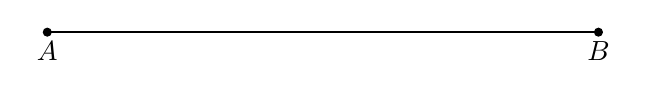
\begin{tikzpicture}
        \draw [-, thick] (0,0)--(7,0);
        \draw [fill] (0,0) circle [radius=0.05] node[below]{$A$};
        \draw [fill] (7,0) circle [radius=0.05] node[below]{$B$};
      \end{tikzpicture}
      \end{center}

\newpage

\item Given line segment $\overline{AB}$ with midpoint $M$, that is, $\overline{AM} \cong \overline{BM}$. $AB=11.8$. Find the length of $\overline{AM}$.\\[0.75cm]
  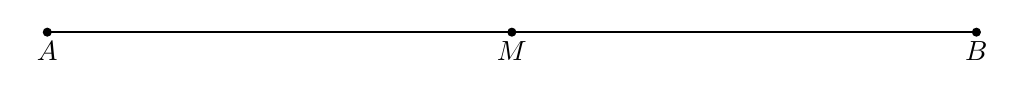
\begin{tikzpicture}
    \draw [-, thick] (0,0)--(11.8,0);
    \draw [fill] (0,0) circle [radius=0.05] node[below]{$A$};
    \draw [fill] (11.8,0) circle [radius=0.05] node[below]{$B$};
    \draw [fill] (5.9,0) circle [radius=0.05] node[below]{$M$};
  \end{tikzpicture}
\vspace{3cm}

\item Given $\overline{AMB}$, $M$ bisects $\overline{AB}$, $AM=2x-10$, $BM=x+2$. Find ${AB}$.\\
Complete all the steps for full credit. \smallskip
  \begin{enumerate}
    \item Sketch and label the situation
    \item Write an equation
    \item Solve for $x$
    \item Answer the question
    \item Check your solution
  \end{enumerate}

\vspace{4cm}

\item Given that $S$ bisects $\overline{RT}$. $RT=7x-3$, $ST=2x+6$. Find ${RT}$.\\
Complete all the steps for full credit.

\end{enumerate}
\end{document}